\chapter{Introducción}
\newpage

Además de como gestor de contenido, Drupal también puede funcionar sirviéndose de contenido externo 
a través de otras aplicaciones Web, tales como Twitter, Facebook o Google. Esta comunicación entre 
Drupal y aplicaciones externas es lo que hace del primero una potente plataforma de gestión 
de contenido, tanto propio como ajeno. Por ejemplo, un desarrollador Drupal puede alimentar su aplicación
con contenido a través de \emph{Aggregation} o \emph{feeds RSS}. 

Uno de los métodos más robustos para utilizar contenido externo es el módulo 
\emph{FeedAPI (Application Programming Interface)} ya que permite fácilmente utilizar RSS 
para ser usado desde Drupal. Otro módulo importante para la integración de Drupal con servicios Web es 
\emph{Service} ya que nos ayudará a conectarnos con servicios Web utilizando diferentes protocolos, como
XMLRPC, JSON, JSON-RPC, REST, SOAP y AMF. En este sección revisaremos cómo interactuar nuestro sitio Drupal
utilizando estas interfaces.

En esta sección además aprenderemos:

\begin{itemize}
  \item ¿Qué son los servicios Web y para qué se utilizan?
  \item ¿Para qué y cómo utiliza Drupal servicios Web?
  \item Drupal como proveedor y consumidor de servicios
  \item Normas para desarrollar y utilizar servicios Web.
\end{itemize}

\section{¿Qué son los servicios Web?}

Para conseguir que nuestro sitio Drupal se comunicque e interactue con otras aplicaciones web como
Facebook, Twitter o Google, necesitamos utilizar una ser de protocolos estándares de comunicación, 
llamados servicios web. Los servicios web proporcionan interactuación y comunicación entre aplicaciones 
web tanto remota como localmente. Es decir, podemos utilizar servicios web de Flickr para importar todas 
nuestras fotografías de estas vacaciones, en nuestra aplicación Drupal.

Las llamadas a servicios Web ocurren a través de protocolos cifrados y son traducidos en un lenguaje
estándar que son comprendidos por ambas partes, utilizando normalmente XML para este propósito. 
XML es un formato basado en texto, por lo que casi todos los sistemas informáticos y las aplicaciones 
pueden trabajar con dicho formato.

El protocolo de servicios Web está basado en un concepto conocido como \textbf{Remote Procedure Calling (RPC)}
que permite a una aplicacion inicializar o ``llamar'' a una función dentro de una aplicación que se 
encuentra en un servidor remoto. Por ejemplo, nuestro sitio Drupal puede llamar a un servicio Web de 
Twitter para obtener nuestros últimos tweets y publicarlos automáticamente en nuestro sitio, o 
moverlos a nuestro tablón de Facebook, utilizando los servicios Web de este último.

\subsection{XML y Servicios Web}

Como se ha mencionado, los servicios Web utilizando el lenguaje de marcado XML para comunicarse.
Nuestra aplicación Drupal y el proveedor de servicios Web utilizando el protocolo estándar de comunicación 
HTTP para enviarse mensajes utilizando el lenguaje XML. Se utiliza XML porque es un lenguaje común entre 
todos las aplicaciones Web y éste reemplaza al lenguaje propietario en el que el servicio Web fue escrito
y el protocolo de comunicación que utilice. Así las aplicaciones se entienden más fácilmente. Quizás se 
entienda mejor con esta analogía: si dos personas, un Español y un Ruso hablan entre si y ninguno conoce 
el lenguaje del otro, lo usual es hablar un lenguaje que hablen ambos, como el Inglés. 

Algunos ejemplos de protocolos de comunicación con servicios Web que veremos en el capítulo son:
\begin{itemize}
  \item SOAP (Simple Object Access Protocol), 
  \item UDDI (Universal Description, Discovery and Integration),
  \item WSDL (Web Services Description Language),
  \item XML-RPC (XML Remote Procedure Call),
  \item JSON (JavaScript Object Notation),
  \item JSON-RPC,
  \item REST (Representational State Transfer) y
  \item AMF (Action Message Format)  
\end{itemize} 

\subsection{El protocolo REST}
El protocolo REST (\textit{Representational State Transfer} o \textit{Transferencia de Estado Representacional}) 
es una técnica para intercomunicar diferentes aplicaciones Web. En él se definen un conjuntos de bases por las cuales
se diseñan servicios Web haciendo teniendo en cuenta los recursos del sistema, el acceso al estado de dichos 
recursos y cómo se transfieren por HTTP hacia clientes escritos en diversos lenguajes. La principal 
característica de REST es la simplicidad, calidad por la que logró desbancar a SOAP y las interfaces basadas 
en WSDL.

Los pilares de REST son:

\begin{itemize}
  \item utiliza métodos de HTTP para comunicarse.
  \item no mantiene estado.
  \item utiliza URIs como si se tratase de directorios.
  \item se comunica a través de mensajes escritos tanto en XML, JSON o ambos.
\end{itemize}

Un ejemplo de la potencia y facilidad con la que trabajamos utilizando REST la podemos encontrar en la integración 
de Drupal con Twitter: podemos pedir los últimos \textit{tweets} de una cuenta, recibirlos y mostrarlos en 
nuestra aplicación Drupal. Para ello, pediremos este contenido a través de una petición GET a una URI 
de Tweet, que nos responderá con el contenido en formato XML o JSON, el cual ya podremos procesar y 
utilizar en nuestra aplicación. 
 
\begin{figure}
  \centering
    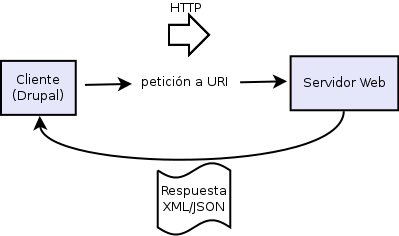
\includegraphics{Assets/Introduccion/Imagenes/diagrama_servicios_web.png}
  \caption{Ejemplo de Rest}
\end{figure}

\section{¿Son útiles los servicios Web para Drupal?}
Está claro que si lo que necesitamos es utilizar contenido de otras aplicaciones Web, necesitamos hacer 
uso de servicios Web. Debido a la interoperabilidad de éstos, podemos comunicar nuestra aplicación Drupal 
con cualquier otra aplicación, sea Drupal o no. Utilizando Drupal como proveedor de servicios Web, además 
podremos compartir nuestro contenido con el resto del mundo y no será específico de nuestro sitio.
 
Integrando, por ejemplo, nuestra aplicación Drupal con Picassa, podemos subir automáticamente todas las 
fotos que utilicemos en nuestro sitio a un álbum público, consiguiendo ser indexados también a través de 
nuestras imágenes. Otro ejemplo lo podemos tener con Linkedin: utilizando los servicios de la famosa red de 
profesionales podremos compartir contenido de nuestra aplicación a nuestro perfil, directamente  

Además, podemos servirnos de datos externos para hacer nuestro sitio más rico: podemos utilizar servicios 
de un centro metereológico o utilizar la herramienta de traducción o los mapas de Google para 
convertir nuestra aplicación en un sitio robusto y funcional. 

\section{¿Cómo utiliza Drupal servicios Web?}

Drupal puede utilizar los protocolos que antes mencionamos, incluyendo SOAP, REST y XML-RPC, así como 
servirse de servicios cuyos mensajes hayan sido codificados usando RSS y XML. Para ello, se pueden escribir 
clientes de comunicación propios o utilizar el módulo \textit{Services} o cualquier otro módulo de integración 
con servicios. Pero primero veámos cómo funciona Drupal como un consumidor de servicios Web, es decir, 
cómo consume Drupal recursos de un servidor Web externo.



 